% Security and safety net for TrackOne
\section{Security and Safety Net}
\label{sec:security}

This section summarises the threat model, security goals, plausible attacks, critical failures we wish to avoid, and the concrete countermeasures that TrackOne implements or recommends. The text deliberately focuses on the evidence pipeline: collection and aggregation of telemetry facts into daily blobs, deterministic Merkle batching and day roots, anchoring into the OpenTimestamps (OTS) ecosystem (public or stationary calendars), storage of proofs and metadata, and independent verification via \texttt{verify\_cli.py}. Physical attacks on sensors, network confidentiality, and full SIL/IEC 61508 compliance are out of scope for TrackOne; ADR-022 frames operational constraints and traceability for deployments.

\subsection{Scope}
We reason about the security of the TrackOne evidence pipeline from ingestion through long-term verifiability. Specifically included:
\begin{itemize}[nosep]
  \item Collection and aggregation of telemetry / canonical facts into per-day blobs and Merkle trees (\texttt{facts/}, \texttt{day/*.bin}, \texttt{blocks/}).
  \item Construction and storage of per-day records (\texttt{day/YYYY-MM-DD.json}, \texttt{day/YYYY-MM-DD.bin}) and Merkle roots (\texttt{day\_root}).
  \item Anchoring of \texttt{day\_root} into the OTS ecosystem (public calendars or a stationary calendar per ADR-014).
  \item Storage and management of OTS proofs (\texttt{*.ots}) and OTS metadata sidecars (\texttt{*.ots.meta.json}).
  \item Verification tooling and CI automation that declares evidence ``verified'' (\texttt{verify\_cli.py}, CI tox envs, ADR-022 operational checks).
\end{itemize}

Out of scope: physical extraction of device keys, side-channel attacks, network-layer confidentiality (we focus on integrity, authenticity, and non-repudiation), and formal SIL certification.

\subsection{Security goals}
We group goals into three categories: Integrity \& Authenticity, Availability \& Robustness, and Operational Trust.

\subsubsection{Integrity and authenticity}
\begin{enumerate}[nosep]
  \item Immutable history: once a day's facts are committed and the day\_root anchored, it should be infeasible to change, reorder, or delete entries without detection by auditors.
  \item Authentic anchors and proofs: an accepted \texttt{day\_root} or OTS proof must be provably produced from the intended aggregation and correspond to an on-chain (Bitcoin) commitment at or before the claimed time.
  \item Tamper evidence: any post-hoc modification of \texttt{day.bin}, \texttt{day.json}, block headers, proof files (\texttt{*.ots}), or proof metadata (\texttt{*.ots.meta.json}) must be detectable by verification tooling and schema/consistency checks.
\end{enumerate}

\subsubsection{Availability and robustness}
\begin{enumerate}[nosep]
  \item Graceful degradation: temporary unavailability of public calendars or a stationary calendar must not corrupt ledger state; such days are recorded as \emph{pending anchor} and surfaced clearly to operators.
  \item Reproducibility and auditability: independent verifiers can recompute a day's root from published facts and validate OTS proofs against Bitcoin headers using only published artifacts, schemas, and verifier tools.
\end{enumerate}

\subsubsection{Operational trust}
\begin{enumerate}[nosep]
  \item Honest CLI semantics: when \texttt{verify\_cli.py} reports success, all relevant checks (Merkle, schema, OTS proof) have passed; skipped checks are clearly marked and reflected in exit codes.
  \item Configuration safety: calendar configuration mistakes (mixing test and prod, pointing at malicious calendars) must be hard to perform silently; misconfiguration should be observable in logs/metrics and fail safe.
\end{enumerate}

\subsection{Plausible attacker models}
We categorize adversaries by capability rather than actor name.
\begin{itemize}[nosep]
  \item \textbf{A1 — Network adversary:} can intercept, replay or block traffic to calendar servers and can host arbitrary calendar endpoints (spoofed or malicious calendars).
  \item \textbf{A2 — Storage adversary / insider:} can modify or delete files in storage (facts, day blobs, proofs, meta) but cannot break standard cryptographic primitives.
  \item \textbf{A3 — Malicious operator / misconfiguration:} can change environment variables, CI markers, or point verification at incorrect roots; may also disable tests accidentally or intentionally.
  \item \textbf{A4 — Buggy or compromised calendar:} a calendar that returns inconsistent proofs, signs incorrect commitments, or equivocates across clients.
\end{itemize}

\subsection{Representative attack scenarios}
The table below summarises representative attacks (AT-*) used to reason about countermeasures and failure modes.

\begin{table}[ht]
\centering
\caption{Representative attack scenarios (AT-*)}
\begin{tabular}{p{3cm}p{4cm}p{8cm}}
\toprule
\textbf{Attack} & \textbf{Adversary} & \textbf{Description / strategy} \\
\midrule
AT-1: Post-hoc tampering & A2 (storage / insider) & Modify \texttt{day.bin} or constituent facts after anchoring; attempt to reuse or forge proofs to keep verification green. \\

AT-2: Proof substitution (``stuffing'') & A2 / A1 & Copy a valid \texttt{.ots} from another artifact and rename it to match the target day; rely on superficial verifier checks that only test file presence. \\

AT-3: Calendar equivocation & A1 / A4 & Run or compromise calendars that present different proof views to different verifiers (split-view), or return proofs for commitments not reflected on main Bitcoin chain. \\

AT-4: CI / operator misconfiguration & A3 & Change CI markers or env vars so OTS/TSA checks are skipped or stubbed in CI while workflows still report green. \\

AT-5: Metadata corruption / loss & A2 / non-malicious failure & Delete or corrupt \texttt{*.ots.meta.json} files making it ambiguous which proof corresponds to which artifact or whether an upgrade occurred. \\
\bottomrule
\end{tabular}
\end{table}

\subsection{Critical failures}
We define top-level critical failures (CF-*) whose occurrence we must prevent or detect early.
\begin{itemize}[nosep]
  \item \textbf{CF-1: False positive verification (silent integrity failure).} \texttt{verify\_cli.py} returns success while the underlying facts or day blob differ from what was anchored. This undermines trust and risks regulatory exposure.
  \item \textbf{CF-2: Undetected calendar misbehavior.} A calendar equivocates or returns invalid proofs but verification tooling accepts them, compromising long-term verifiability.
  \item \textbf{CF-3: Loss or ambiguity of proof history.} Proof and meta files are deleted or corrupted in ways that make it impossible to reconstruct the chain of custody for certain days.
  \item \textbf{CF-4: Safety net disabled by misconfiguration.} CI or CLI is misconfigured so critical tests are skipped or stub modes are silently used in production, allowing regressions to land.
\end{itemize}

All design choices and countermeasures are evaluated against these failure modes.

\subsection{Countermeasures and mapping to failures}
The following groups the primary design choices and maps them to attacks and failures they mitigate.

\subsubsection{Cryptographic structure and canonicalization}
\begin{itemize}[nosep]
  \item Deterministic Merkle trees (canonical JSON, sorted leaves) and stable hashing are the primary integrity primitives (ADR-003, ADR-006). They ensure that any change to \texttt{day.bin} changes the root and will be detected by recomputation.
  \item Enforce that \texttt{day.bin} is the canonical artifact used for hashing and stamping; \texttt{day.json} is retained for human inspection but not treated as the authoritative hash input.
\end{itemize}

\subsubsection{OTS proof sidecars and metadata schema}
\begin{itemize}[nosep]
  \item Store proofs as sidecar files (\texttt{day/YYYY-MM-DD.bin.ots}) and separate, validated metadata files (\texttt{proofs/YYYY-MM-DD.ots.meta.json}) that include at minimum: artifact SHA-256, artifact path, OTS file path, calendar info, client version and timestamps.
  \item The verifier recomputes artifact SHA-256 and compares to the meta file before attempting OTS verification; this prevents naive proof substitution (AT-2) and aids recovery when metadata is inconsistent (AT-5).
\end{itemize}

\subsubsection{Stationary calendar and configuration patterns}
\begin{itemize}[nosep]
  \item Use a stationary calendar for CI and predictable local verification (ADR-014): this reduces flakiness and makes equivocation easier to detect in controlled contexts.
  \item Distinguish modes via explicit envvars: \texttt{OTS\_STATIONARY\_STUB} for fast local tests, \texttt{OTS\_CALENDARS} to point at stationary or public calendars, and \texttt{RUN\_REAL\_OTS} to gate slow tests. Treat stub mode as non-production and require an explicit opt-in for production runs.
\end{itemize}

\subsubsection{Verification logic and tooling}
\begin{itemize}[nosep]
  \item \texttt{verify\_cli.py} follows a strict sequence: recompute SHA-256 of \texttt{day.bin} => compare to meta => check block header/merkle root => run OTS verify. Any mismatch aborts with a non-zero exit code.
  \item Exit codes and human-readable messages differentiate between: missing artifact, hash mismatch, OTS missing, OTS invalid, and calendar unavailability. This prevents silent success (CF-1, CF-4).
\end{itemize}

\subsubsection{Testing, CI and schema validation}
\begin{itemize}[nosep]
  \item JSON schemas for block headers, day records, and \texttt{ots.meta.json} are enforced in CI. Tests include negative mutation tests: deliberately corrupt \texttt{day.bin} or change proof meta and assert verification failures.
  \item Tox/CI contracts require that OTS-related tests run in an explicit env (e.g., \texttt{ots-cal} or \texttt{real\_ots}) and that PRs touching verification code include tests; missing tests or skipped markers cause CI to fail (ADR-022 operational policy).
\end{itemize}

\subsubsection{Operational controls and enumerations}
\begin{itemize}[nosep]
  \item Periodic enumerations and archival scripts check for orphaned \texttt{.ots} files, missing \texttt{.meta.json} pairs, and report anomalies as CI/monitoring alerts. This helps detect CF-3 and AT-5 early.
  \item Site-specific operator playbooks (ADR-022) require a 72-hour pilot, staged rollouts, and explicit thresholds (storage, data loss) that trigger operator intervention rather than silent failure.
\end{itemize}

\subsection{Mechanism mapping (summary table)}
\begin{table}[ht]
\centering
\caption{Mechanism mapping: attacks/failures to countermeasures}
\begin{tabular}{p{3cm}p{5cm}p{6cm}}
\toprule
\textbf{Attack / Failure} & \textbf{Countermeasure} & \textbf{Mechanism} \\
\midrule
AT-1 / CF-1 (post-hoc tampering) & Merkle canonicalization; \texttt{day.bin} canonical; recompute+hash check & Any change to \texttt{day.bin} changes Merkle root; \texttt{verify\_cli} recomputes hashes and rejects mismatched proofs. \\
\addlinespace
AT-2 (proof substitution) & Meta schema + hash binding & Meta ties an artifact path and SHA to a proof; wrong proof = hash mismatch = reject. \\
\addlinespace
AT-3 / CF-2 (calendar equivocation) & Stationary calendar + explicit calendar config + logs & Stationary calendar yields deterministic proof behaviour in CI; logs and metrics expose equivocation or anomalies before acceptance. \\
\addlinespace
AT-4 / CF-4 (CI misconfig) & Tox env contracts, required markers, ADR-022 policies & CI fails PRs that remove or skip critical verification tests; markers gate \texttt{real\_ots} runs. \\
\addlinespace
AT-5 / CF-3 (meta loss) & Periodic enumerations, schema validation, archival scripts & Scripts detect missing meta/proof pairs and alert operators; backups and retention policies preserve proof history. \\
\bottomrule
\end{tabular}
\end{table}

\subsection{Opportunity and Risk matrices}

\begin{table}[ht]
\centering
\caption{Opportunity matrix: benefits and leverage points for TrackOne}
\begin{tabular}{p{3cm}p{8.5cm}p{2.5cm}}
\toprule
\textbf{Opportunity} & \textbf{Description} & \textbf{Impact} \\
\midrule
Predictable audits & Deterministic canonicalization + public anchoring enables low-cost third-party audits and reproducible evidence trails. & High \\
\addlinespace
Stationary calendar & Local calendar reduces CI flakiness and provides deterministic proof upgrade behaviour for integration testing. & Medium \\
\addlinespace
Peer attestation & Operator peer signatures provide immediate provenance and short-term assurance ahead of blockchain confirmation. & High \\
\addlinespace
Low marginal cost & Daily batching amortises anchoring cost across many facts, making long-term deployment economically feasible. & High \\
\bottomrule
\end{tabular}
\end{table}

\begin{table}[ht]
\centering
\caption{Risk matrix: primary risks, likelihood, and mitigation priority}
\begin{tabular}{p{3cm}p{5.5cm}p{2cm}p{2.5cm}}
\toprule
\textbf{Risk} & \textbf{Description} & \textbf{Likelihood} & \textbf{Priority} \\
\midrule
False-positive verification & Verify CLI reports OK despite artifact tampering or proof mismatch & Low-Medium & High \\
\addlinespace
Calendar equivocation & Malicious or compromised calendar returns inconsistent proofs & Low & High \\
\addlinespace
Metadata loss / orphaned proofs & Missing or corrupted meta/json makes proof association ambiguous & Medium & Medium \\
\addlinespace
CI/Operator misconfiguration & Skipped \texttt{real\_ots} tests or stubbed mode used in prod & Medium & High \\
\addlinespace
Hardware failure modes & Sensor drift, electrode corrosion leading to mis-measurement & Medium-High & Medium \\
\bottomrule
\end{tabular}
\end{table}

\subsection{Risk/opportunity landscape matrix}

\begin{figure}[ht]
\centering
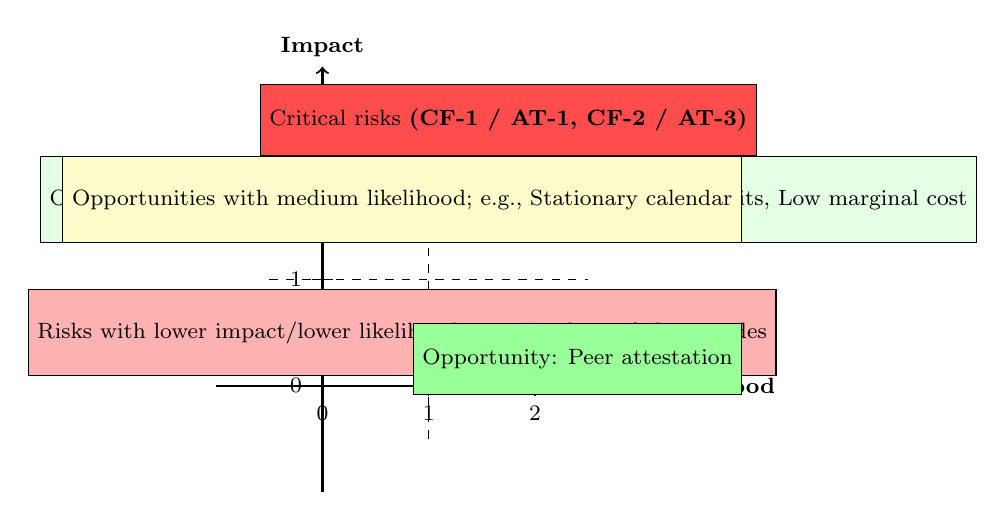
\begin{tikzpicture}[scale=0.9, every node/.style={font=\footnotesize}, x=1.5cm, y=1.5cm]
  % grid
  \draw[->, thick] (-1,0) -- (3,0) node[right]{\textbf{Likelihood}};
  \draw[->, thick] (0,-1) -- (0,3) node[above]{\textbf{Impact}};
  \foreach \x in {0,1,2} { \draw (\x,0.1) -- (\x,-0.1) node[below]{\x}; }
  \foreach \y in {0,1,2} { \draw (0.1,\y) -- (-0.1,\y) node[left]{\y}; }
  \draw[dashed] (1, -0.5) -- (1, 2.5);
  \draw[dashed] (-0.5, 1) -- (2.5, 1);
  % quadrants
  \node[draw, align=center, fill=green!10, minimum width=2.8cm, minimum height=1.1cm] at (1.75,1.75) {Opportunities \textnormal{(High impact, high likelihood)}; e.g., Predictable audits, Low marginal cost};
  \node[draw, align=center, fill=yellow!20, minimum width=2.8cm, minimum height=1.1cm] at (0.75,1.75) {Opportunities with medium likelihood; e.g., Stationary calendar};
  \node[draw, align=center, fill=red!10, minimum width=2.8cm, minimum height=1.1cm] at (1.75,0.5) {Risks with medium impact; e.g., Metadata loss};
  \node[draw, align=center, fill=red!30, minimum width=2.8cm, minimum height=1.1cm] at (0.75,0.5) {Risks with lower impact/lower likelihood; e.g., Hardware failure modes};
  % highlight high priority
  \node[draw, align=center, fill=red!70, minimum width=2.2cm, minimum height=0.9cm] at (1.75,2.5) {Critical risks \textbf{(CF-1 / AT-1, CF-2 / AT-3)}};
  \node[draw, align=center, fill=green!40, minimum width=2.2cm, minimum height=0.9cm] at (2.4,0.25) {Opportunity: Peer attestation};
\end{tikzpicture}
\caption{Visual matrix of likelihood vs impact for TrackOne risks and opportunities.}
\label{fig:risk-opportunity-matrix}
\end{figure}

\subsection{Discussion and limitations}
We explicitly acknowledge the remaining risks and limits:
\begin{itemize}[nosep]
  \item TrackOne does NOT provide SIL-level guarantees; it is a verifiability-first evidence pipeline. When the system is later used for automated actuation, a separate safety case and certification effort will be required.
  \item We rely on Bitcoin as a long-lived root of trust; extreme systemic failures (large-scale chain reorgs, long-term protocol changes) would affect proof semantics. Mitigations include multi-protocol anchoring (TSA) and strong meta bookkeeping (ADR-015).
  \item Operational correctness requires disciplined deployment: misconfigured calendars or CI that treats stubbed OTS as production can undermine the safety net. ADR-022 and CI contracts mitigate this by making pilot/staging explicit and by failing PRs that lower test coverage or gate markers.
\end{itemize}
